\section{Side Result: Products Of Rotated Regular Polygons}
\label{sec:rotated-regular-polygons}

This section studies Lagrangian products of rotated regular polygons. The
theorem-strength result is for the one-parameter pentagon family
\[
  K_\theta = P_5 \times_L R(\theta)P_5 \subset \mathbb{R}^2_q \oplus \mathbb{R}^2_p,
\]
where \(P_5\) is the regular pentagon with circumradius \(1\), and
\(R(\theta)\) is the counterclockwise rotation in the second Lagrangian factor.
The Haim--Kislev--Ostrover counterexample is a member of this family
\cite{HaimKislevOstrover2024}. The result below identifies the entire
one-dimensional profile of the systolic ratio in this family.

\subsection{Empirical curves}
\label{subsec:rotated-regular-polygons-empirical-curves}

The regular polygon products provide a structured test family between the
single HKO example and the higher-dimensional searches in the rest of the
thesis. For two regular polygons \(P_n\) and \(P_m\), we sampled
\[
  P_n \times_L R(\theta)P_m
\]
over a mesh of rotation angles and computed the EHZ capacity using the finite
polytope algorithm from Section~\ref{sec:quadratic-program-algorithm-hk2019}.
The sampled data are not used in the proof below. They were useful because the
pentagon-pentagon curve suggested a simple formula and isolated the midpoint
angle \(\theta=\pi/10\).

\begin{figure}[htbp]
  \centering
  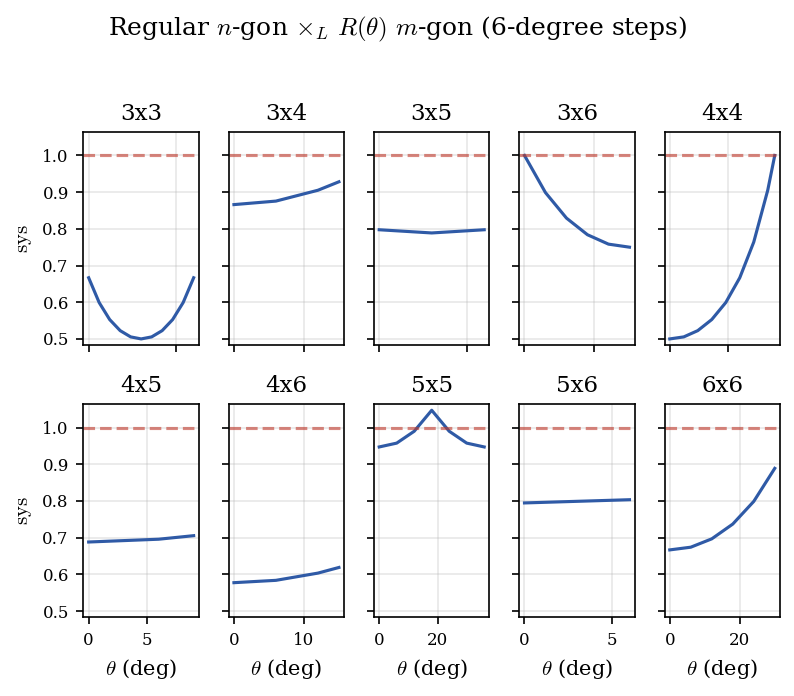
\includegraphics[width=0.88\linewidth]{working/rotated-regular-polygons/lagrangian-products-polygon-pairs.png}
  \caption{Sampled systolic ratios for several rotated regular polygon
  products. The broad sweep gives context for the pentagon theorem: most tested
  pairs stay below \(1\), while the \(5\times 5\) family exhibits the HKO-type
  peak above \(1\). This figure is empirical motivation only.}
  \label{fig:rotated-regular-products-pairs}
\end{figure}

\begin{figure}[htbp]
  \centering
  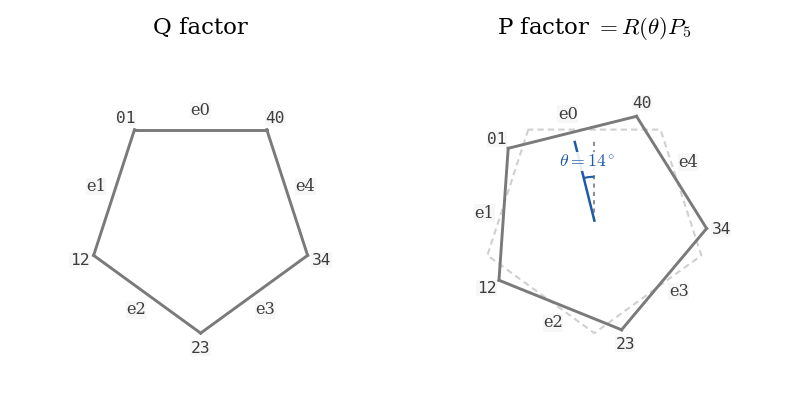
\includegraphics[width=0.78\linewidth]{working/rotated-regular-polygons/labeled-pentagons-theta.png}
  \caption{The two regular pentagons and the rotation parameter \(\theta\).
  The first pentagon lies in the \(q\)-factor. The second pentagon is rotated
  in the \(p\)-factor.}
  \label{fig:rotated-pentagons-theta}
\end{figure}

\begin{figure}[htbp]
  \centering
  
\includegraphics[width=0.82\linewidth]{working/rotated-regular-polygons/lagrangian-products-5x5.png}
  \caption{Sampled systolic ratio for the rotated pentagon product. The
  sampling suggested the secant-squared profile proved below. The figure is
  empirical motivation only; the proof uses the finite-candidate reduction and
  an executable certificate for the resulting exact algebraic checks.}
  \label{fig:rotated-pentagons-curve}
\end{figure}

The empirical sweep also served a negative role: it was not satisfying as a
final argument. Several three-bounce branches remain close enough to the
candidate branch that a proof by plotting or by a short list of hand
calculations would be fragile. The exact computation in the proof replaces that
manual case analysis by symbolic classification of the finite candidate list
from the proof below. Here the bounce count is the block count in the
enumeration; a block may contain an adjacent pair of facets.

\begin{figure}[htbp]
  \centering
  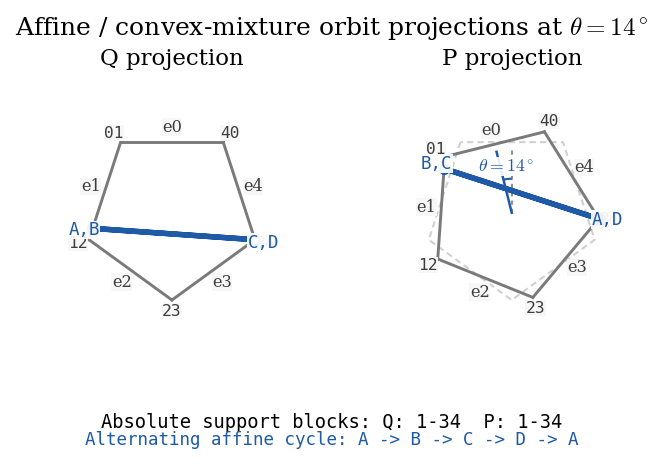
\includegraphics[width=0.78\linewidth]{working/rotated-regular-polygons/trajectory-projections-theta14-affine.png}
  \caption{Projection of a representative minimizing orbit at a sampled angle.
  The figure shows the geometry of the active branch; it is not part of the
  lower-bound certificate.}
  \label{fig:rotated-pentagons-orbit-projection}
\end{figure}

\subsection{Formula for the pentagon product}
\label{subsec:rotated-regular-polygons-formula-for-the-pentagon-product}

For a real number \(\theta\), define
\[
  d(\theta)
  :=
  \min_{k\in\mathbb{Z}}\left|\theta-\frac{k\pi}{5}\right|.
\]
Then \(0\le d(\theta)\le\pi/10\).

\begin{theorem}[Rotated pentagon product]
\label{thm:rotated-pentagon-product-formula}
Let \(P_5\subset\mathbb{R}^2\) be the regular pentagon with circumradius \(1\),
and let \(K_\theta=P_5\times_L R(\theta)P_5\). Then, for all
\(\theta\in\mathbb{R}\),
\[
  \operatorname{sys}(K_\theta)
  =
  \frac{5+2\sqrt{5}}{10}\sec^2(d(\theta)).
\]
In particular, the maximum in this one-parameter family is attained exactly at
the angles with \(d(\theta)=\pi/10\), where
\[
  \operatorname{sys}(K_\theta)=\frac{3+\sqrt{5}}{5}>1.
\]
\end{theorem}

\begin{proof}
The proof has three parts. First, symmetries reduce the theorem to the
half-domain \(0\le\theta\le\pi/10\). Second, an explicit branch gives the
required upper bound for the capacity, and hence for the systolic ratio. Third,
we reduce the corresponding lower bound on the open half-domain to finitely
many exact algebraic checks, and verify those checks by an executable SageMath
certificate. Continuity fills the remaining cut points and the endpoints. At
the end, we apply the initial symmetry reduction to return from the half-domain
to all real \(\theta\).

The family is periodic with period \(2\pi/5\): simultaneous rotation of both
factors is symplectic, and the two pentagons are invariant under rotation by
\(2\pi/5\). Reflection gives the usual reduction to
\([0,\pi/5]\). There is one further symmetry because the two factors are the
same odd regular polygon: the symplectic map \(-J_0\) swaps the factors and
sends
\[
  P_5\times_L R(\theta)P_5
  \quad\text{to}\quad
  R(\theta)P_5\times_L(-P_5).
\]
After a simultaneous rotation by \(-\theta\), and using
\(-P_5=R(\pi)P_5=R(\pi/5)P_5\) modulo the \(2\pi/5\)-symmetry of the pentagon,
this becomes \(P_5\times_L R(\pi/5-\theta)P_5\). Thus it is enough to prove
\[
  \operatorname{sys}(K_\theta)
  =
  \frac{5+2\sqrt{5}}{10}\sec^2\theta
  \qquad
  \text{for }0\le\theta\le\frac{\pi}{10}.
\]

We now compute the candidate branch on this half-domain. In the raw-sigma
notation used below, this is the branch
\[
  (3,8,1,0,5,6).
\]
Solving the KKT equations for this branch gives the action
\[
  c_{\mathrm{act}}(\theta)
  =
  \left(1+\cos\left(\frac{\pi}{5}\right)\right)^2\sec\theta .
\]
The four-volume is independent of \(\theta\), since rotation preserves area in
the second factor:
\[
  \operatorname{vol}_4(K_\theta)
  =
  \operatorname{area}(P_5)^2,
  \qquad
  \operatorname{area}(P_5)
  =
  \frac{5}{2}\sin\left(\frac{2\pi}{5}\right).
\]
Therefore the active branch gives
\[
  \frac{c_{\mathrm{act}}(\theta)^2}{2\operatorname{vol}_4(K_\theta)}
  =
  \frac{\left(1+\cos\left(\frac{\pi}{5}\right)\right)^4}
       {2\operatorname{area}(P_5)^2}\sec^2\theta
  =
  \frac{5+2\sqrt{5}}{10}\sec^2\theta .
\]
This proves the required upper bound for \(\operatorname{sys}(K_\theta)\) on
the half-domain, since the EHZ capacity is the minimum action.

It remains to prove the lower bound on the open half-domain. By the
finite-candidate reduction from
Section~\ref{sec:quadratic-program-algorithm-hk2019}, this is enough to verify
a finite collection of exact algebraic statements for the two- and
three-bounce candidates described below. The verification is implemented in
SageMath. The successful run is not an independent proof of the theorem; it is
the executable certificate that the finite checks required by this reduction
all pass.

The source and full transcript are in
\path{experiments/regular-products/pentagon-rotation-formula-proof/}:
\begin{itemize}
  \item \path{executable_proof.sage.py},
  \item \path{executable_proof.full.stdout.txt}.
\end{itemize}
The script computes the active branch in the same exact framework: the function
\texttt{assert\_formula\_checks} solves the KKT branch for the intended sigma,
asserts the displayed capacity formula for that branch, and checks the constant
used to convert it to the systolic-ratio formula.

The certificate uses the parameter
\[
  t=\tan(\theta/2).
\]
The unrotated pentagon already has coefficients in the real subfield of
\(\mathbb{Q}(\zeta_{20})\), and the identities
\[
  \sin\theta=\frac{2t}{1+t^2},
  \qquad
  \cos\theta=\frac{1-t^2}{1+t^2}
\]
make all branch expressions rational functions of \(t\) over that coefficient
field. Sage uses exact algebraic root isolation to compare roots and endpoints
inside the interval \(0<t<\tan(\pi/20)\).

The finite-candidate theorem from
Section~\ref{sec:quadratic-program-algorithm-hk2019} applies to this family.
Thus it is exhaustive to consider the two- and three-bounce candidates; all
other combinatorial types are either redundant or cannot realize a smaller
action. In the Lagrangian product
\(P_5{}_q\times_L R(\theta)P_5{}_p\), the relevant facet sequence alternates
between \(q\)-blocks and \(p\)-blocks. We label the \(q\)-facets
\(0,\ldots,4\) and the \(p\)-facets \(5,\ldots,9\), in counterclockwise order
in each factor.

A block is either one facet or an ordered adjacent pair of facets inside one
factor. For a \(k\)-bounce candidate, where \(k=2\) or \(k=3\), Sage chooses
\(k\) non-overlapping \(q\)-blocks and \(k\) non-overlapping \(p\)-blocks. It
fixes one \(q\)-block as the first block, orders the remaining \(q\)-blocks and
all \(p\)-blocks, and then alternates \(q\)- and \(p\)-blocks cyclically. The
final raw sigma is obtained by concatenating the facets inside those blocks.
Thus the alternation is block-by-block, not necessarily facet-by-facet.
For code simplicity, the implementation keeps raw ordered representatives
instead of quotienting by cyclic shifts, reversals, or symmetries. This
overcounts rather than undercounts.

Before solving KKT systems, Sage applies exact transition pruning on the open
half-domain. Same-factor transitions must have nonempty facet intersection.
Mixed \(q/p\)-transitions must also have the positive symplectic transition
sign, and Sage checks that this sign has no interior cut point on the open
half-domain. Thus a pruned-out raw sigma fails a necessary transition condition
throughout the open half-domain. The rest of the Sage computation then
classifies every raw representative that survives this pruning.

\Needspace{22\baselineskip}
The following excerpt is the Sage enumeration loop for one value of \(k\). The
helper \texttt{blocks} returns singleton facets and ordered adjacent pairs; the
helper \texttt{non\_overlapping\_selections} keeps only selections with no
repeated facet.
\begin{minted}{python}
def enumerate_k_bounce_sigmas(k):
    q_blocks = blocks(Q_FACETS)
    p_blocks = blocks(P_FACETS)
    for q_selection in non_overlapping_selections(q_blocks, k):
        for p_selection in non_overlapping_selections(p_blocks, k):
            for q_rest_perm in permutations(range(k - 1)):
                for p_perm in permutations(range(k)):
                    sigma = []
                    sigma.extend(q_selection[0])
                    sigma.extend(p_selection[p_perm[0]])
                    for round_index in range(1, k):
                        sigma.extend(
                            q_selection[1 + q_rest_perm[round_index - 1]]
                        )
                        sigma.extend(p_selection[p_perm[round_index]])
                    yield tuple(sigma)
\end{minted}

For each raw sigma that passes the open-domain transition pruning, Sage solves
the KKT system exactly. When a branch exists, this gives rational functions for
the multipliers \(\beta_i\), the quadratic value \(Q_\sigma\), and the action
gap
\[
  \frac{1}{2Q_\sigma} - c_{\mathrm{act}}(\theta).
\]
The script then cuts the open interval at all roots and poles of these
functions. On each resulting cell, signs are constant. Sage checks one exact
algebraic sample point per cell. Thus the strict inequalities
\[
  \beta_i>0,\qquad Q_\sigma>0,\qquad
  \frac{1}{2Q_\sigma}-c_{\mathrm{act}}(\theta)>0
\]
are decided by exact algebraic computation, not by numerical sampling.

The classifier is an ordered chain of proof exits. For each raw sigma, one of
the following accepted cases must occur.
\begin{enumerate}
  \item The KKT system is inconsistent.
  \item \(Q_\sigma\) is identically zero.
  \item The KKT system is singular, but every solution has some multiplier
    forced to be identically zero, so no strictly feasible branch exists.
  \item The action gap is identically zero; this is a tie with the active
    branch, not a lower competitor.
  \item No open cell has all \(\beta_i>0\) and \(Q_\sigma>0\), so the branch is
    nowhere strictly feasible on the open half-domain.
  \item On every feasible open cell, the action gap is strictly positive.
\end{enumerate}
The script also has a manual-review fallback for unrecognized cases. That
fallback is not accepted by the certificate; the script asserts that every
classified raw sigma lands in one of the accepted exits.

\Needspace{17\baselineskip}
The following slightly elided excerpt shows the fail-closed part of the full
certificate loop. The full source file is the proof source; this listing is
included only to make the control flow visible in the thesis.
\begin{minted}{python}
def run_preflight():
    ...
    sigmas = transition_pruned_sigmas_open()
    assert len(sigmas) == EXPECTED_OPEN_SIGMA_COUNT
    ...
    return sigmas

def run_certificate(progress_every, limit=None):
    all_sigmas = run_preflight()
    sigmas = all_sigmas if limit is None else all_sigmas[:limit]
    for index, sigma in enumerate(sigmas):
        classification = classify_sigma(sigma, min_action)
        ...
        assert classification.status in ACCEPTED_STATUSES
    ...
    if limit is None:
        print(f"CERTIFICATE PASSED in {elapsed:.2f}s")
\end{minted}

\begin{figure}[htbp]
  \centering
  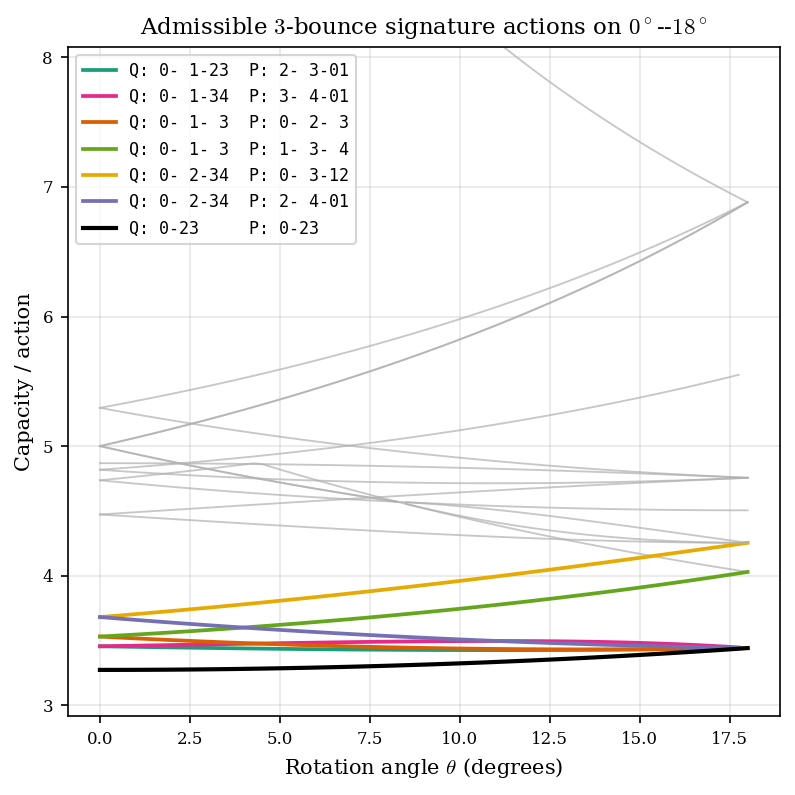
\includegraphics[width=0.78\linewidth]{working/rotated-regular-polygons/three-bounce-branch-actions.png}
  \caption{Sampled actions of several three-bounce branches that motivated the
  exact finite classification. The figure is diagnostic and empirical; the
  lower bound in the theorem uses the exact finite classification implemented
  in Sage.}
  \label{fig:rotated-pentagons-three-bounce-actions}
\end{figure}

The full run reports
\[
\begin{aligned}
  \texttt{open\_domain\_raw\_sigma\_count} &= 3340,\\
  \texttt{classified\_raw\_sigma\_count} &= 3340,
\end{aligned}
\]
Here \(3340\) is the full unquotiented list after open-domain transition
pruning, not a sampled subset. The same number of raw sigmas is then classified
by the certificate. The run then prints
\[
  \texttt{CERTIFICATE PASSED in 2126.34s}.
\]
The status counts in that run were
\[
\begin{array}{rcl}
  \texttt{no\_kkt\_solution} &=& 25,\\
  \texttt{zero\_q\_identity} &=& 1680,\\
  \texttt{singular\_kkt\_forced\_zero\_beta} &=& 470,\\
  \texttt{not\_feasible\_on\_open\_domain} &=& 735,\\
  \texttt{zero\_gap\_identity} &=& 20,\\
  \texttt{strict\_gap\_positive\_on\_feasible\_open\_domain} &=& 410.
\end{array}
\]
These counts are not separate mathematical input; they are the transcript of
the exact finite certificate. The mathematical conclusion is that, on every
open cell of the exact cell decomposition of \(0<\theta<\pi/10\), no feasible
HK/KKT branch has action below the active branch.

Together with the active branch, equality holds on every open cell. The path
\(\theta\mapsto K_\theta\) is continuous in the Hausdorff topology, the EHZ
capacity is continuous on convex bodies in this topology, and the volume is
constant. Hence \(\operatorname{sys}(K_\theta)\) is continuous in \(\theta\).
Since the displayed formula is continuous as well, equality on the open cells
extends to the cut points and to the endpoints \(0\) and \(\pi/10\). This
proves the formula on the half-domain. The symmetry reduction at the beginning
of the proof then gives the theorem for all real \(\theta\).
\end{proof}
